\section{The Digital Back-end and The First Digital Prototype}\label{sec:digital_prototype}
The digital system of the Q-Pix readout begins when the first digital data are recorded.
This occurs during the collection of a recorded timestamp in response to the logic reset pulse sent from the Schmitt Trigger from analog front-end.
These triggers are a sent as the response from a build up of charge on a pixel in a LArTPC (Section~\ref{sec:lartpcs}).
An example of a pixel ring with a connected ASIC are shown in Figure~\ref{fig:qpix_asic_introduction}.

This record happens in response any one, or more, of the pixels, which for the first ASIC prototype is up to 16.
The timestamp is the value of a local 32-bit counter at the time the ASIC receives the reset pulse.
When a trigger is sent from any pixel the data recorded are local counter as well as the input level of all pixels ('1' indicates high, '0' indicates low).

\begin{figure*}[t!]
\centering
\begin{subfigure}[t]{.5\textwidth}
  \centering
  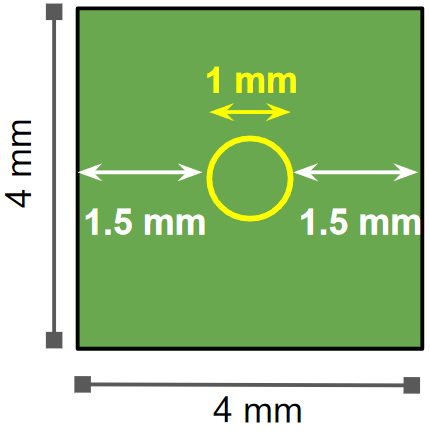
\includegraphics[width=0.5\textwidth]{images/single_pixel_dimensions_qpix.png}
  \caption{Charge Collection Pixel}
\end{subfigure}%
~
\begin{subfigure}[t]{.5\textwidth}
  \centering
  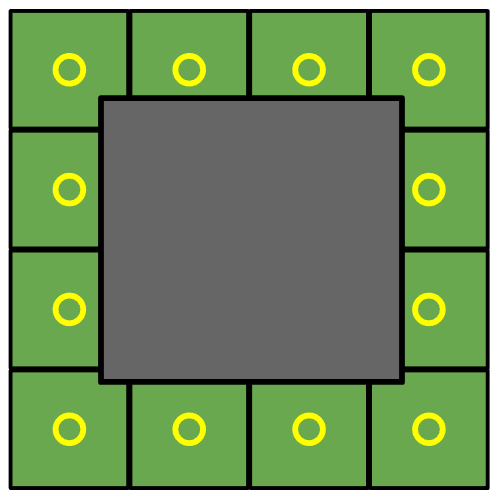
\includegraphics[width=0.5\textwidth]{images/single_asic_dimensions_qpix.png}
  \caption{Q-Pix ASIC connected to 4$\times$4 pixels}
\end{subfigure}
\caption{Each Q-Pix ASIC (b) is expected to connect to up 16 pixels (a) within the LAr.
The dimensions of each pixel are 4$\times$4~\unit{mm^2}, where the collection ring has a diameter of 1~\unit{mm}.
Each ASIC supports up to a maximum of 16 channels, or pixels.
}
\label{fig:qpix_asic_introduction}
\end{figure*}

The full Q-Pix digital back-end is a collection of interconnected ASICs that form tiles.
Tiles are then connected to controlling nodes as shown in Figure~\ref{fig:qpix_tile_introduction}, indicated by the colored boxes.
In order for the system to work each ASIC must be able to send and receive data, which are routed to and from its tile via the controlling nodes.
The sheer number of pixels required for an DUNE-FD 10 kT module require an extremely reliable means of charge and time calibration, stable buffer depths, and protection against single-point failure (SPF).

\begin{figure}[]
\centering
\begin{subfigure}[t]{.5\textwidth}
  \centering
  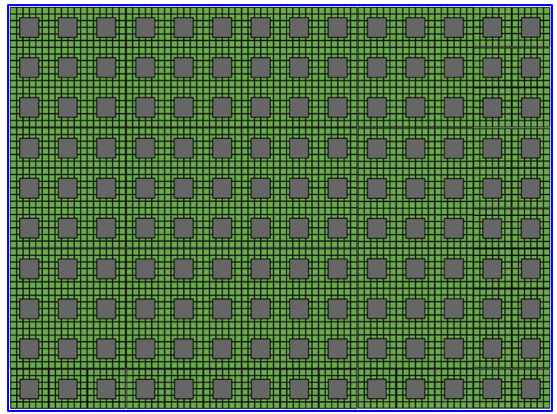
\includegraphics[width=0.6\textwidth]{images/single_tile_qpix.png}
  \caption{A single tile of 10$\times$14 Q-Pix ASICs}
\end{subfigure}%
\begin{subfigure}[t]{.5\textwidth}
  \centering
  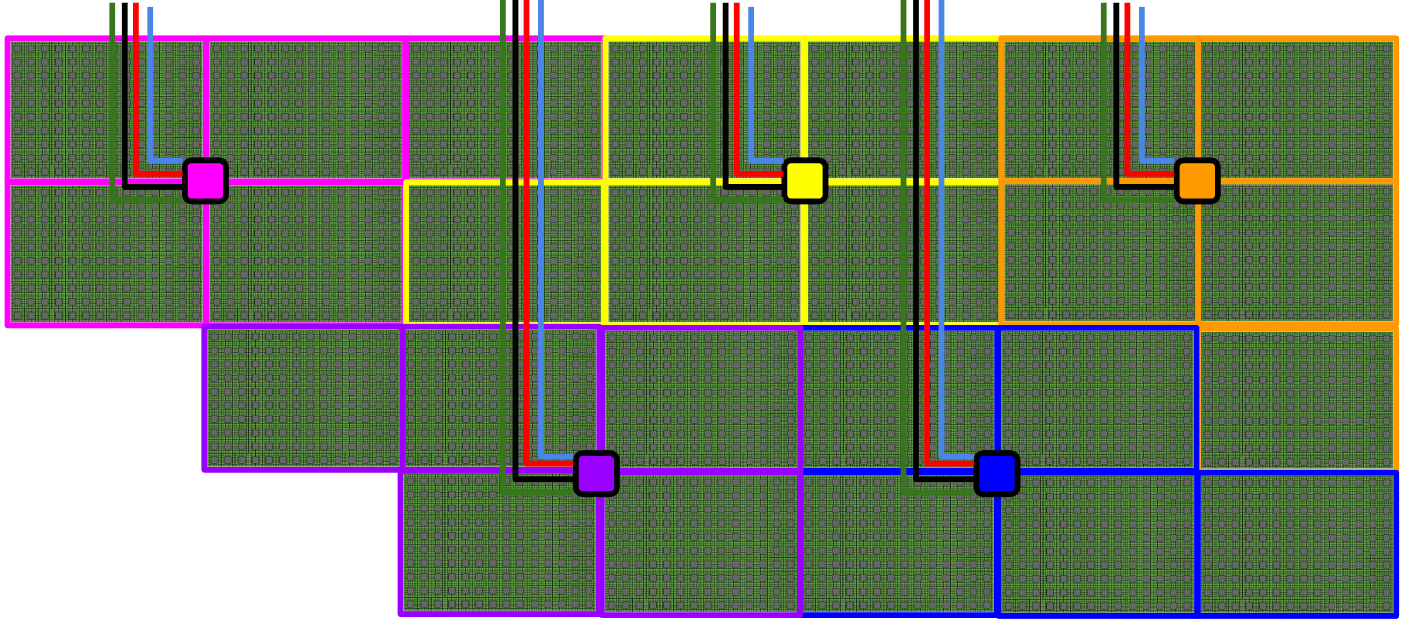
\includegraphics[width=0.85\textwidth]{images/array_of_tiles_qpix.png}
  \caption{An array of inter-connected tiles.}
\end{subfigure}
\caption{A modular tile (a) of Q-pix ASICs can be inter-connected (b) to create a larger charge collection plane. 
The highlighted nodes in (b) indicate possible locations aggregator nodes to interconnect multiple tiles from a single controlling node.
These aggregators can connect power, clock, ground, and data out of the full detector which are represented by the four colored traces leaving the tile array.
}
\label{fig:qpix_tile_introduction}
\end{figure}

The logical components of each ASIC are represented in Figure~\ref{fig:qpa_diagram}.
These components are responsible for controlling the basic features of the ASIC including communications, configuration, and data collection.
Data communication between ASICs is of primary consideration, since all recorded data must be transmitted between ASICs, through aggregators, and eventually to a storage disc.

\begin{figure}[]
\centering
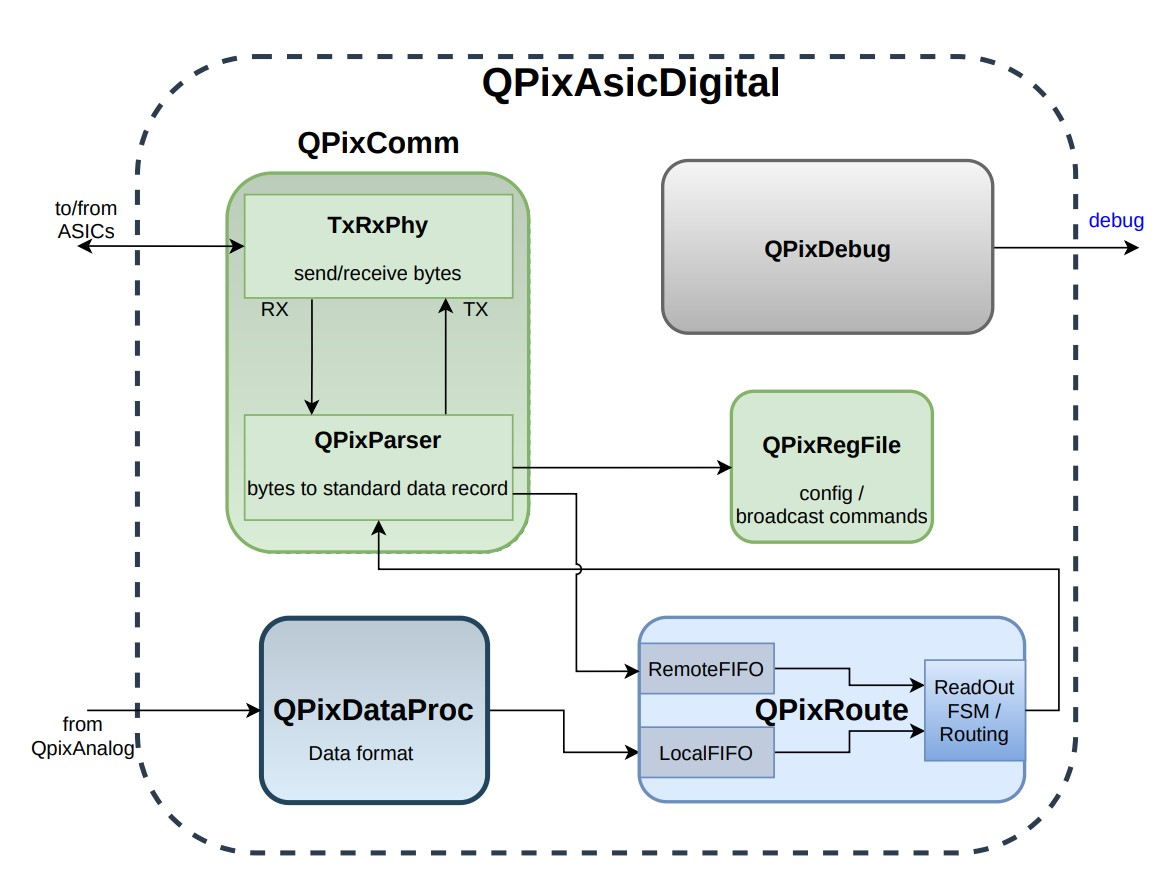
\includegraphics[width=0.9\textwidth]{images/digital_node_overview.jpg}
\caption{Diagram of the different components of the digital node.
  Shown are the different sections of the control logic for the ASIC: QpixComm, QPixDataProc, QPixRoute, and QPixRegFile.
  The QpixComm layer is responsible for routing packets between the physical layer and handles the parsing of incoming data packets.
  The QpixDataProc layer is responsible for recording timestamp data during a reset from the analog front-end.
  The QpixRegFile contains configuration information, such as routing, ASIC location, and the timestamp counter.
  QPixRoute determines the controlling state machine that, based on register configurations, determines what packets are sent to which neighboring nodes.
  The Remote and Local FIFOs determine the packet memory of the ASIC. 
  The QpixDebug layer connects internal signals (such as the local oscillator) to external pins for planned futures tests of the ASIC prototype.
  }
\label{fig:qpa_diagram}
\end{figure}

The QPixComm module describes the communication layer of the ASIC, and determines how to communicate with the ASIC, described in Section~\ref{sec:endeavor}.
To allow flexible communications, each transaction is capable of being encoded to serve different functions within the ASIC.
Each ASIC is able to determine its appropriate response to a packet based on its contents; this procedure is described in Section~\ref{sec:digi_packets}.

Dynamic programming of remote routing is a key feature of the Q-Pix back-end design.
Although each ASIC currently supports the ability to route itself, the results of Chapter~\ref{chap:sim} indicate that routing updates of a tile are better suited to the aggregator.
The controlling node can update a register within any ASIC to purposefully direct it's routing.
Each ASIC is also capable of determining its location within a tile, as well as controlling its routing via register information, described by the QpixRegFile block.
We provide further detail the various control registers in Section~\ref{sec:registers}.

Finally, the data collection module, QPixDataProc, controls how the ASIC records triggers sent from the analog front-end.
We describe the ASIC's response to pixel triggers in Section~\ref{sec:data_collection}


\subsection{Inter-ASIC communication via endeavor protocol}\label{sec:endeavor}
The data must be transmitted between ASICs.
Since one design feature of the Q-Pix readout require that the ASICs have independent oscillators, the communication between neighbors is necessarily asynchronous.
Each ASIC permits up to four neighbor connections as shown in Figure~\ref{fig:example_connections}.

\begin{figure}[]
\centering
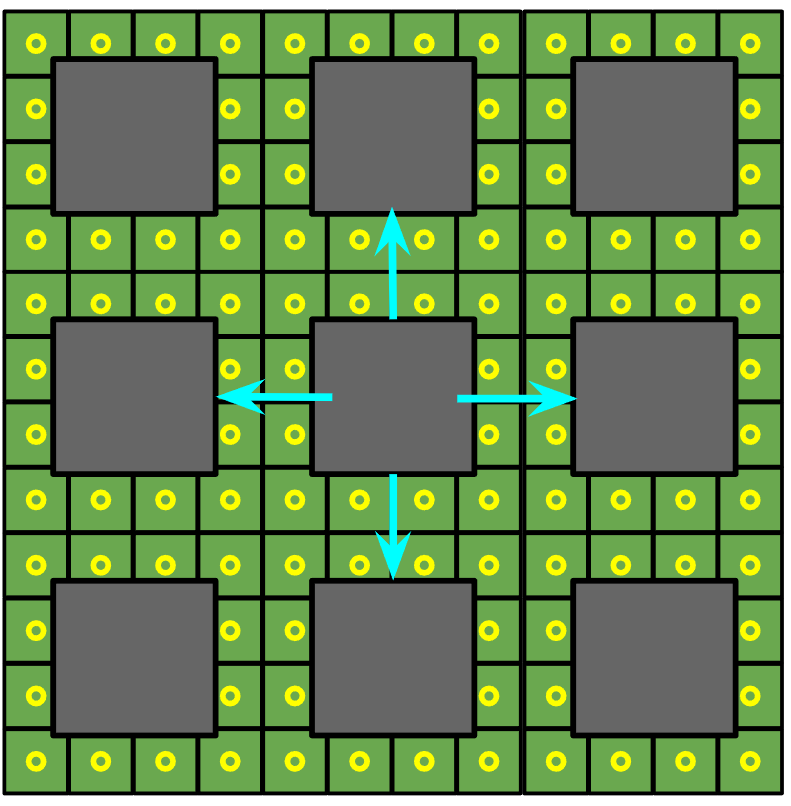
\includegraphics[width=0.5\textwidth]{images/asic_neighbor_connections_qpix.png}
\caption{Every ASIC permits connections to its neighbors in the cardinal directions.
Each connection is two pairs of differential connections which permit asynchronous data transfer.
Four connections of two pairs of differential connections require a total of 16 PCB traces to fully connect an ASIC to four neighbors.
}
\label{fig:example_connections}
\end{figure}

The asynchronous communication protocol used is called an "Endeavor" protocol, which was originally developed for the Asynchronous Multi-ASIC Communication version 2 (AMACv2) ASIC.
The endeavor protocol was specifically designed for high-speed asynchronous data communication between neighbor ASICs.
An example of a transmission of data using this protocol is shown in Figure~\ref{fig:endeavor}.

\begin{figure}[]
\centering
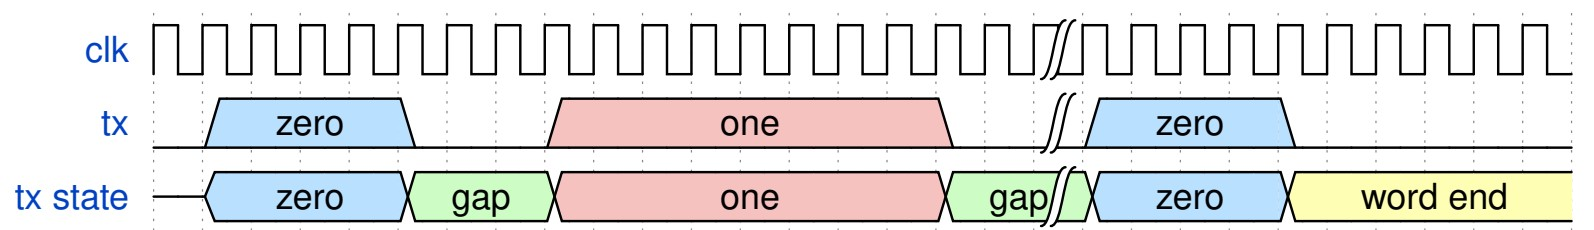
\includegraphics[width=\textwidth]{images/endeavor_protocol.jpg}
\caption{Diagram of the endeavor transmission (Tx) protocol.
The primary components of the endeavor protocol involve how long the transmitter (Tx) drives the signal high.
The receiver (Rx) counts how long each signal is driven high, then based on the count it determines whether the transmitter intended to send a '1' or a '0' bit.
The convention used in the prototype ASIC sends a '1' bit for twice the number of clock cycles it will send a '0' bit.
After a bit is sent, there is a gap period where the Tx preps the Rx for another bit.
The conclusion of the transmission occurs after 64 bits have been sent, where the Tx holds the signal low for longer the a normal gap word indicating the packet is complete.
}
\label{fig:endeavor}
\end{figure}

Data are sent one bit at a time following the procedure shown in Figure~\ref{fig:endeavor}. 
The procedure follows that a Tx drives the transmission line high for a variable time to send either a One ('1') or a Zero ('0') bit.
After each bit is sent, the Tx drives the line low for a period known as the 'Gap'.
A transaction is complete when 64 bits have been sent, and the Tx drives the line low for a longer period known as 'Finish'.
The range of clocks for acceptable states are described in Table~\ref{tab:endeavor_parameters}.

We refer to a completed transaction of data between neighbor ASICs as a "packet".
For simplicity, each ASIC expects that every data transaction will send (and therefore receive) exactly 64 bits.
A packet is constructed where the first bits that are sent are the "lowest bits" of the packet.

The ASIC reads the packet by first inspecting the "type" of the packet, which are controlled by "packet header".
The packet header bits are the four bits sent as the 57th through 60th bits in the packet.
We refer to "bit location" as the order of the bit sent in the Endeavor transaction, where the packet sends the 1st bit, and concludes with the 64th bit.
There are four bit locations shared by all packets:

\begin{itemize}
    \item Y Location of sending ASIC: 33--36
    \item X Location of sending ASIC: 37--40
    \item Packet Header: 57--60
    \item Unused Bits, but required for valid packet: 61--64
\label{bit_reservation}
\end{itemize}

When an ASIC receives a valid packet, the ASIC enables a valid signal.
The packet is handled based on the bits within the header of this packet.
How the packet is handled is determined the by the packet header~\ref{bit_reservation}.

If the packet originated from the aggregator node then this packet is treated as a broadcast.
Broadcast commands record unique numbers associated with this request and are also sent to all connected neighbors except from the direction that the broadcast is received.
A unique broadcast number is used to avoid registering the same request.

If the packet was not from an aggregator node then this packet is treated as "remote packet" from a neighbor node.
All data transfers of any kind are treated so that all communication happens between individual nodes and an aggregator node.
Therefore, any packet that originates on a node that isn't the aggregator node will be sent to the aggregator node.
The direction of that this packet is sent is determined by the configuration register.

\begin{table}
\begin{center}
\begin{tabular}{||p{20mm} p{20mm} p{20mm} p{20mm} p{60mm}||}
 \hline
 Bit & Allowed\newline Minimum & Allowed\newline Maximum & Sent by Tx & Purpose \\ [0.5ex]
 \hline\hline
 Zero & 4 & 12 & 8 & Number of Clock cycles Tx drives signal high to send a '0' bit. \\
 \hline
 One & 16 & 32 & 24 & Number of Clock cycles Tx drives signal high to send a '1' bit. \\
 \hline
 Gap & 8 & 32 & 16 & Determines range of clock cycles Tx should drive low to pause between next bit. \\
 \hline
 Finish & 40 & None & 40 & Determines minimum number of clock cycles Tx should drive signal to indicate packet is complete. \\
 \hline
\end{tabular}
\caption{The parameters of the Endeavor protocol used by the Q-Pix digital prototype discussed in this thesis.
The column 'Sent by Tx' indicates how many clock the Tx will sent during each step.
The Zero and One bits indicate the number of clock cycles that the Tx line should drive the signal high to send a '1' or a '0' bit, respectively.
The Gap and Finish are used to prep the Rx to receive the next data bit or to indicate the packet has finished. 
The ASIC will only accept packets that contain exactly 64 bits.
An example of this protocol in use is shown in Figure~\ref{fig:endeavor}.
}
\label{tab:endeavor_parameters}
\end{center}
\end{table}


One important note about the Endeavor protocol is that the transaction time of the packet is not constant.
The number of clocks required to send a '1' bit differs from the number of clocks for a '0' bit.
However, it is straight forward to show that the number of clocks the Tx will use to send a packet is give by:
\begin{equation}~\label{eq:endeavor_clocks}
  N_{clocks} = N_{One}N_{1} + N_{Zero}N_{0} + 64N_{gap} + N_{finish}
\end{equation}

Where $N_{1}$ and $N_{0}$ refer to the number of bits within the 64 bit sequence will be '1' and '0' respectively.
The values $N_{one}, N_{Zero}, N_{gap}$ and $N_{finish}$ can be taken from Table~\ref{tab:endeavor_parameters}.
However since each packet must contain four zero unused bits, and $60 = N_{1} + N_{0}$, Equation~\ref{eq:endeavor_clocks} can be rewritten as:

\begin{equation}
  N_{clocks} = 24(60 - N_{0}) + 8N_{0} + 64*16 + 40
\end{equation}

If we assume the average packet has equal high bits and low bits, $N_{0} = 30 + 4$, the average clocks in a transaction is:
\begin{equation}~\label{eq:avg_packet}
  N_{avg} = 24*28 + 8*34 + 64*16 + 40 \sim 2000 
\end{equation}


\subsection{Types of Packets}\label{sec:digi_packets}
How each digital node responds to a successful packet transaction depends on the packet header.
One primary development goal for the Q-Pix digital ASIC is to make the simplest design possible that achieves its goals.
To this end, there are only four different types of packets words used, as shown in Figure~\ref{fig:datum}.

\begin{figure}[]
\centering
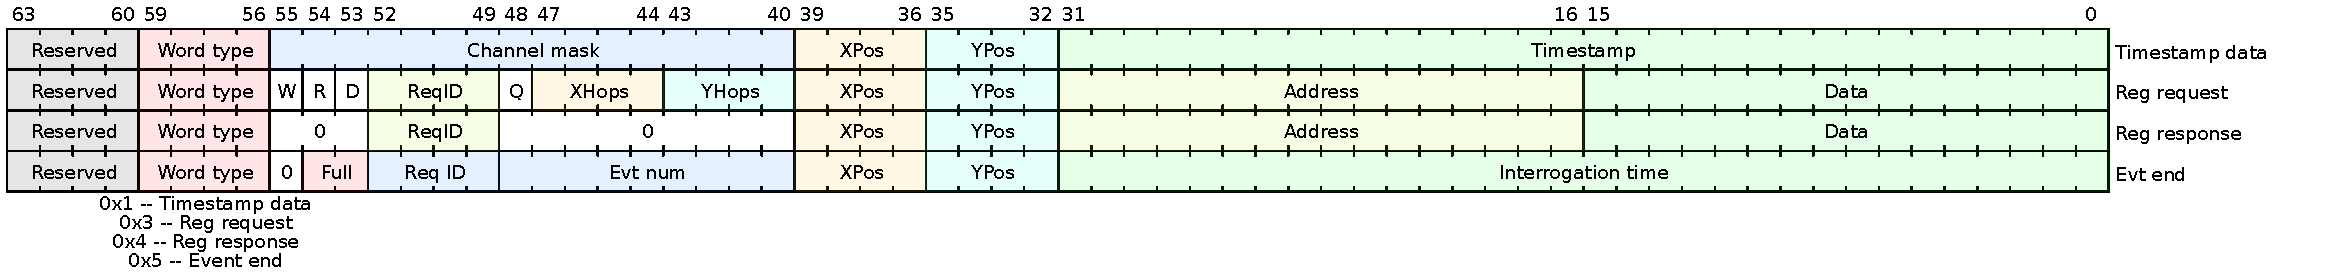
\includegraphics[width=\textwidth]{images/qpix_word_format.pdf}
\caption{Example of Datum words and their allocation as currently implemented in the simulation and first prototypes.
The two types of data packets (Table~\ref{tab:packet_data}) are timestamp data and event end data which are used to record reset times and interrogation times respectively.
The interrogation time is described in Section~\ref{sec:local_data_packet}.
The Register Request packet is special because it can only be created by an aggregator node, described in Table~\ref{tab:packet_register}. 
The Register response is created and sent back to the aggregator node in response to a request,.
}
\label{fig:datum}
\end{figure}

The timestamp and event end packets are created by each ASIC and represent true data for analysis.
The Register Request and Register Response packets indicate communication between an ASIC and an aggregator.

The Register Request is a special packet that can only be created by an aggregator node; The Q-Pix digital ASIC can not create a Register Request packet.
This packet contains a special bit (48) that indicates if this packet came from the aggregator node, and is only valid on the first ASIC which sees this packet.
If this packet is configured as a broadcast (See Section~\ref{sec:local_data_packet}), or to another node, the ASIC will send this packet identically except with bit 48 ("Q" in Figure~\ref{fig:datum}) held low.

The Register Response packet is created by an ASIC to send to an aggregator node upon a register read request from an aggregator.
When an ASIC receives a packet that isn't a register request, it knows that this packet did not originate from the aggregator node, and therefore handles these packets identically, described in Section~\ref{sec:digital_fsm}.

\subsection{Configuration Registers}\label{sec:registers}
The configuration of the digital node is handled through local registers.
These registers can only be updated when an ASIC receives a Register Request from an aggregator node.

These registers are described within QpixRegFile module, shown in Figure.~\ref{fig:qpa_diagram}.
These registers include the ability to control routing of data packets, reset, enable, and channel masking.
Table~\ref{table:node_registers} describes the implemented register addresses and their functions:

\begin{table}
\begin{center}
\begin{tabular}{||p{30mm} p{30mm} p{90mm}||}
 \hline
 Address & Name & Function \\ [0.5ex]
 \hline\hline
  0x01 & Command & four bits are used to select hard and soft interrogations, full ASIC reset, or transfer reset, respectively. \\
 \hline
  0x03 & Routing & one bit toggle and four bit selection of direction to send data, otherwise dynamic. \\
 \hline
  0x04 & Channel Mask & 16 bit mask selection of triggers from input pixels. \\
 \hline
  0x05 & Position & 8 Bit selection of data to determine ASIC position within tile. \\
 \hline
  0x06 & Disable & Four bit selection of which neighbor node inputs are ignored. \\
 \hline
  0x07 & Local Disable & Single bit selection to stop collecting data when sending. \\
 \hline
\end{tabular}
\caption{The address values are not sequential because some registers have become deprecated through development.
The command register controls for resets and triggers (interrogations) for data.
The Routing controls either dynamic or manual routing.
}
\label{table:node_registers}
\end{center}
\end{table}

The composition of any register word is shown in Table~\ref{tab:packet_register}.
Each of the registers in Table~\ref{table:node_registers} are accessed by setting the correct address value in the register request packet.
\begin{table}
\begin{center}
\begin{tabular}{|| p{30mm} | p{30mm} | p{90mm} ||}
 \hline
 Bit Location & Name & Function \\ [0.5ex]
 \hline\hline
  0--15 & Data & Excess bits \\
 \hline
  16--31 & Address & Excess bits \\
 \hline
  40--43 & Y Position Transfers & Next Y position in tile. \\
 \hline
  44--47 & X Position Transfers & Next X position in tile. \\
 \hline
  48 & Source Flag & Single Bit flag to indicate whether ot not packet originated from aggregator. \\
 \hline
  49--52 & Request ID & Identifier bits to specify broadcast. \\
 \hline
  53 & Destination Flag & Identifier bit to specify if broadcast is meant for a specific node. \\
 \hline
  54 & Read Flag & Identifier flag to specify if register request is a read. \\
 \hline
  55 & Write Flag & Identifier flag to specify if register request is a write. \\
 \hline
\end{tabular}
\caption{Description of the bit values within the register request word.}
\label{tab:packet_register}
\end{center}
\end{table}

The two essential registers for connecting to and reading from the ASIC are the Routing (0x03) and Command (0x01) registers.
The routing register allows the ASIC to be configured in either a manual or a dynamic routing.
The dynamic routing state allows an ASIC to send its data in the direction it receives a broadcast (Section~\ref{sec:local_data_packet}) from, whereas a manual routing allows the aggregator to predetermine the path of the data words.
The Command register controls both ASIC system resets as well as broadcast types.

\subsection{Local Data Collection}\label{sec:data_collection}
The digital node is responsible for collecting and storing local timestamps in response to pixel resets as well as being able to communicate these data with neighbor nodes.
The node must be able to buffer data so as to prevent packet loss during transactions.
The separation of the remote and local packets are contained within two different FIFOs, as shown in Figure.~\ref{fig:qpa_diagram}.

There are two conditions which must be met in order for a timestamp to be recorded.
First, an incoming reset pulse must be supplied from one of the pixels.
Second, at the time of this incoming reset the corresponding pixel mask must not be set in the channel mask register (See Table~\ref{table:node_registers}).
When both conditions the value of the local reset is recorded into a 32 bit wide FIFO shown in QpixRoute in Figure~\ref{fig:qpa_diagram}.

The composition of the data word is shown in Table~\ref{tab:packet_register}.
\begin{table}
\begin{center}
\begin{tabular}{|| p{30mm} | p{30mm} | p{90mm} ||}
 \hline
 Bit Location & Name & Function \\ [0.5ex]
 \hline\hline
  0--31 & Timestamp & Basic Datum which records the local counter at the time of the reset pulse. \\
 \hline
  32--35 & Y Position & Assigned Y position in tile. \\
 \hline
  36--39 & X Position & Assigned X position in tile. \\
 \hline
  40--55 & Pixel Mask & Pixels which were issuing a reset at this time. \\
 \hline
  56--59 & Word Header & Header value, which is common to all packets. \\
 \hline
  60--63 & Reserved & Unused bits for all packets. \\
 \hline
\end{tabular}
\caption{The 64 bits (starting from zero) which make a Data word.}
\label{tab:packet_data}
\end{center}
\end{table}

\subsubsection{The Local Data Packet and Broadcasts}
\label{sec:local_data_packet}
The transmission of the reset data from the local FIFO to adjacent neighbor nodes begins when an incoming register request from the aggregator is received.
This request is supplied as register request to the command register (Table~\ref{table:node_registers}).
This request may be considered either a ``hard'' or a ``soft'' interrogation command.

The difference between the two types of an interrogation command is whether or not the event end packet is created.
In the case of a ``hard''--interrogation, the event end packet is always created, regardless of the local FIFO.
A Hard Interrogation happens if the first bit of the data written to the command register is high.
In the case of a ``soft''--interrogation, the event end packet is created only if the local FIFO is not empty.
A soft interrogation happens if the second, and not the first, bit of the data written to the command register is high.

The use of two different types of interrogations allows the aggregator control flexibility in how many packets are created during an interrogation.
Interrogations may happen on timescales much more quickly than expected resent pulses ($\mathcal{O}(10^{1}~\unit{s})$, Chapter~\ref{chap:qpix}).
The ability to request data only if available prevents an over abundance of packets which prevents needless data transfers, reduces remote FIFO buildup, and conserves power.

\subsubsection{The Event End Packet}
The event end words perform multiple functions.
First, they may used as checksums to indicate at the aggregator node, or on disk, that this node has successfully transmitted all of its data.
Secondly, the event end word, since it is necessarily 64 bits long, also transmits its own timestamp with the excess bits.
The timestamp that the event end word carries is the time that the time that the node received the broadcast.
This timestamp is used in the frequency calibration of the node; the method for calibration is described in greater detail in Section~\ref{sec:calib}.

\section{The Digital Finite State Machine}\label{sec:digital_fsm}
The Finite State Machine (FSM) of the digital ASIC controls the ASIC's response to packets.
Possible inputs that the ASIC can respond to are timestamps from pixels or communication packets from neighbor ASICs.
Figure~\ref{fig:digital_fsm} shows a representation of the different states as well as the conditions to enter or leave each state.
The two conditions to leave the default (IDLE) state of the ASIC happen when either its remote FIFO is not empty, or it receives a system interrogation (register request packet).

\begin{figure}[]
\centering
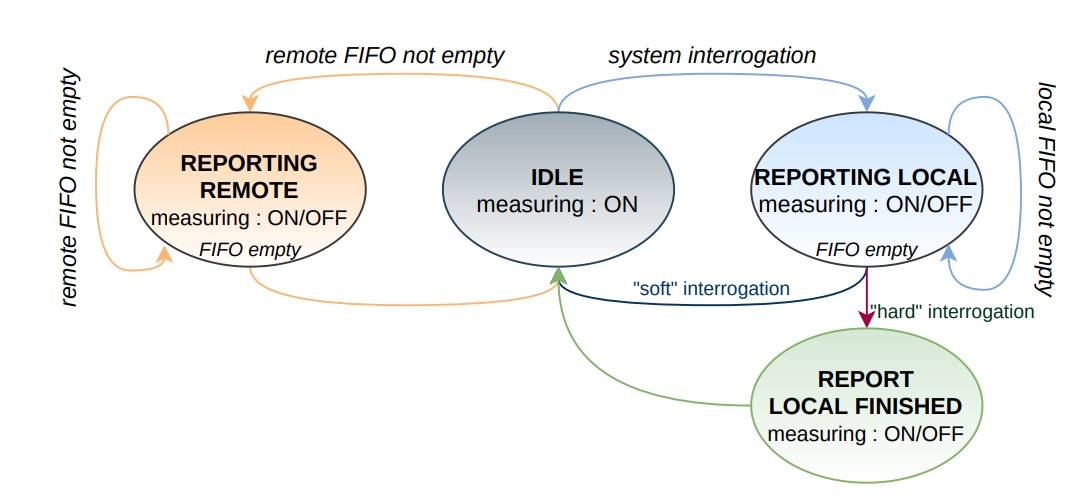
\includegraphics[width=\textwidth]{images/digital_fsm_overview.jpg}
\caption{Diagram of the Digital node's FSM which determines how to respond to incoming packets.
This FSM is defined within the QpixRoute section in Figure~\ref{fig:qpa_diagram}.
The Route FSM determines how and when packets are sent from the ASIC.
}
\label{fig:digital_fsm}
\end{figure}

\begin{itemize}
    \item Idle - Normal ASIC operation.
    \item Transmit Local - Requires soft or Hard Integration from aggregator.
    \item Transmit Finish - Requires Hard Integration or soft integration with available timestamp data.
    \item Transmit Remote - Entered whenever packet received from neighbor that isn't a broadcast.
\end{itemize}~\label{fsm_state_labels}

One of the contributions of this work is to demonstrate how an ASIC that sends data only on the states described in Figure~\ref{fig:digital_fsm} can be used in a large scale LArTPC.
The scale of a DUNE-FD LArTPC requires millions of pixels to run for nearly a decade and requires precision measurements.
To meet these goals, the Q-Pix readout is designed to avoid all potential places of SPF.
One, always unforeseeable, place of failure is correct, but not intended behavior of an ASIC.
To avoid this, we limit, as much as possible, the possible behaviors of the ASIC.

In the next section we discuss the design challenges this ASIC must overcome.

\section{The Digital Back-end problem}\label{sec:digital_problem}
The main objectives of the digital back-end are to correctly measure the data presented to it by the analog front-end and ensure lossless transport of that data to disk.
More simply, the goals of the digital portion of the Q-Pix readout are to record and send data.
We note that the successful completion of these two objectives to be goal of these simulation studies.

Previous sections (\cref{sec:digital_prototype,sec:digital_fsm}) described the design of the current Q-Pix digital ASIC.
This section presents and defends the motivation for this design.

\subsection{The Basic Datum}
We begin with a discussion of the basic datum and mention initial design choices at the physical connection interface.
The structure of this datum determines the buffer widths and depths required to store the data at the local ASIC level as well as the protocol used to transfer this data between ASICs and eventually out of the detector.

The minimum data which the timestamp, the relative location of the ASIC, plus the status of all channels during the timestamp.
Each these factors require bits which must be recorded.

We choose the number of bits for the timestamp ($N_{T}$) to be 32, which prevents frequency wrap-around based on a fast clock frequency.
We choose as the number of bits to assign a location ($N_{loc}$) to be 8, which provides a maximum possible number of unique positions before aggregation to be 256.
Next, since the number of pixels (required by analog front-end design) is 16 we choose this number as the number of bits to represent a ``mask'' ($N_{bits} = 16$).
We need to record all of the channels during each reset since it is technically possible (even if less likely) for multiple analog channels to provide a reset within the same clock window.

We calculate the minimum number of bits per datum to be:
\begin{equation}~\label{eq:nbits_datum}
  N_{bits} = N_{T} + N_{pix} + N_{loc} = 32 + 16 + 8 = 56
\end{equation}

Since buffer memory addresses and widths are normally characterized by powers of two, we can construct the basic datum size above the minimum number of bits provided by~\ref{eq:nbits_datum} to get $N_{datum} = 64$.
The remaining bits are useful for constructing different types of packets to be used by the digital ASICs for additional uses such as register configuration or to provide packet identification.

\subsection{Communication of the Datum}\label{sec:comms}
There exist several asynchronous protocols of communication of digital information.
Some of the differences between protocols exist based on the number of connections between devices and whether or not one pin is allocated to share a clock, etc.
The design of the Q-Pix ASIC limits the number of connections between neighbors to only two.

Our design considerations for this readout include reduction of SPF risk, low power, and minimal electrical routing.
Partly for these reasons, the design choice for communication relies on only two connections between ASICs.
One connection is defined as a data receiver (Rx) and the other as a data transmitter (Tx).
This choice of interface dramatically limits a choice of possible protocols.

The importance of choosing a protocol is to ensure lossless data transmission.
Since every ASIC has its own free running clock, an asynchronous communication protocol is required.
One way to ensure that data can be moved between clocks of different speeds is to stretch the signal or to repeat bits (Figure~\ref{fig:endeavor}).
The more the word is stretched in time, the larger the allowable difference in frequency between the two devices.
However, this lengthening can't proceed indefinitely, otherwise data transmission time would exceed data capture rates.

It is another important design consideration to ensure that transactions proceed as quickly as possibly without data loss.
Additional concerns of long data transactions include the use of more clock cycles which could use more power and increase the risk of electronic noise to leak to the analog front-end during charge collection.
However, these risks can be mitigated if transmission and data acquisition occur at different times.
Our choice of the endeavor protocol is tested in Section~\ref{sec:qdb_prototype}.

Although Endeavor is slower than a traditional Universal Asynchronous Receive Transmitter (UART) protocol, it is stable for approximately double the frequency range: $\approx$ 20\%.
In Chapter~\ref{chap:sim} we show that the overall average packet transaction time is much less ($\sim 0.1\%$) than the wait time between interactions for neutrino events.

\subsection{Buffer Depth Requirements}\label{sec:buffer_requirements}
One feature of a Q-Pix readout is that the amount of memory associated with an event depends on the amount of charge deposited.
The more charge that is deposited, the more resets that are produced.
Each reset corresponds to a new packet to be recorded by the ASIC.
Therefore, the amount of memory than an ASIC has provides a limit to how much charge (energy) it can record within a single event.
The memory for each ASIC is stored in the local and remote FIFOs within the QPixRoute module shown in Figure~\ref{fig:qpa_diagram}.

The major contribution from Chapter~\ref{chap:sim} is to test the required buffer depths for high energy ($\sim$ 10~\unit{GeV}) events in a DUNE-FD LArTPC.
The ice40 FPGAs tested in Section~\ref{sec:qdb_prototype} have a total of 30 Embedded Block Ram models (EBRs).
This allows for a local and remote FIFO depth each of 1024 packets.

\section{Constraining the Digital Back-end Design}\label{sec:digital_constraints}
Section~\ref{sec:qpix_apa} describes how a Q-Pix based hardware readout architecture could fit within a single DUNE-APA.
Here we extend this discussion and use those constraints as the starting point for a search to a solution to the digital back-end architecture.
The first problem to solve is how to aggregate the timestamp data supplied by the large number of pixels ($(\mathcal{O}(10^{6})$) within a DUNE-FD APA.

A Q-Pix architecture will likely use either a high-performance FPGA or a custom ASIC to aggregate data supplied by digital nodes each connected to some number of pixels.
The number of aggregated digital nodes determines the required capabilities of the aggregator node and the selection of an FPGA or ASIC.
Since each additional aggregator node represents an additional SPF risk, our design goal suggests that the optimal configuration is one that produces the least number of aggregator nodes.
Therefore, the goal is to design a routing architecture which is responsible for as many digital nodes as possible for each data aggregator node while still accounting for accurate timing calibration and lossless data acquisition.

In a fully realized design an aggregator might in fact be responsible for multiple tiles, which need not necessarily be the same size.
An aggregator node is required to be capable of sending packets faster than it can receive it so that no data is lost during transmission.
If an aggregator node connects to one ASIC per tile, the average incoming data rate is the number of tiles times the average packet transaction in Equation~\ref{eq:avg_packet}.

The Q-Pix ASIC data rates (8 bytes per $\sim$ 60~\unit{\mu s} = $\sim$ 117~\unit{kBs}) are more than three orders of magnitude slower than the ethernet protocol of the aggregator presented in Section~\ref{sec:qdb_prototype}.
If a Q-Pix ASIC sent data at a rate of 117~\unit{kBs}, and the aggregator can send data via 5~\unit{GB/s} ethernet, a single aggregator could connect to over 40000 tiles without data loss.
For comparison, the dimensions of the DUNE-FD APA in Chapter~\ref{chap:sim} use 862,500 pixels, which would take only 3370 16$\times$16 tiles.

However, as one increases the number of digital nodes per aggregator node one also increases the amount of local oscillators per aggregator, each of which must be calibrated (Section~\ref{sec:calib}).
Additionally, since each digital node requires extra communication time (as discussed in Section~\ref{sec:comms}) the introduction of more channels negatively affects the precision of timing calibrations and potentially increases SPF risk of digital channels.
We consider then that an optimal number of digital nodes per aggregator is one that maximizes the number of digital nodes in a tile but still maintains the required timing calibration and transmits lossless data.

\subsection{Tile Routing Considerations}\label{sec:tile_sim}
A tile is a rectangular array of digital ASICs (nodes) which must provide a path for data from all ASICs (nodes) to the aggregator.
There is one special node within the tile that connects to the aggregator.
This special node we refer to as the ``base-node'' as all data and instruction commands, regardless of routing, must pass through this node.
The symmetry of the rectangular tile allows any corner node to be the base node, and we choose the upper-left to define a convention.
An example of a tile with a corner base-node is shown in Figure~\ref{fig:cbn}.

\begin{figure}[]
\centering
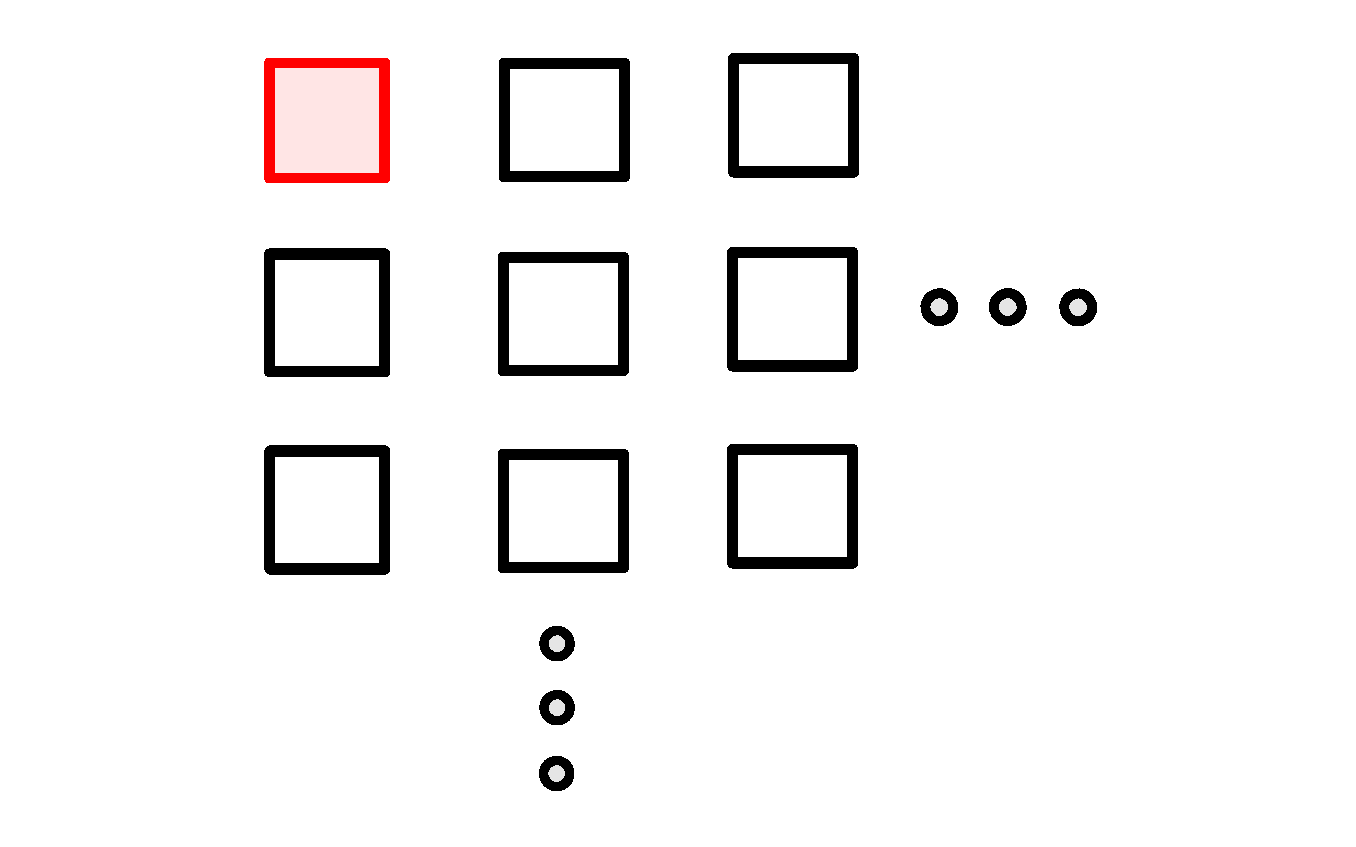
\includegraphics[width=0.8\textwidth]{images/CBN.pdf}
\caption{Example of an Corner Base-Node configuration.
The base-node is colored and highlighted in red.
The base-node (ASIC) is the special node which is the only ASIC that connects to the aggregator. 
All data paths, regardless of routing must pass through this node.
}
\label{fig:cbn}
\end{figure}

The most robust protection a tile can have is to be fully connected, which allows the maximum number of unique paths from the base node to any other node.
Each path (Tx or Rx connection) is as an edge between nodes.

Here we introduce a particular representation for a tile which is useful for simplifying simulations and for analyzing particular routing configurations.
The most general tile configuration occurs when all adjacent nodes are connected; this creates what we refer to as a ``fully connected tile'' (FCT).
An example of a FCT is shown in Figure~\ref{fig:fc_tile}.
Any particular choice of an effective routing must then be a subset of this fully connected version.

\begin{figure}[]
\centering
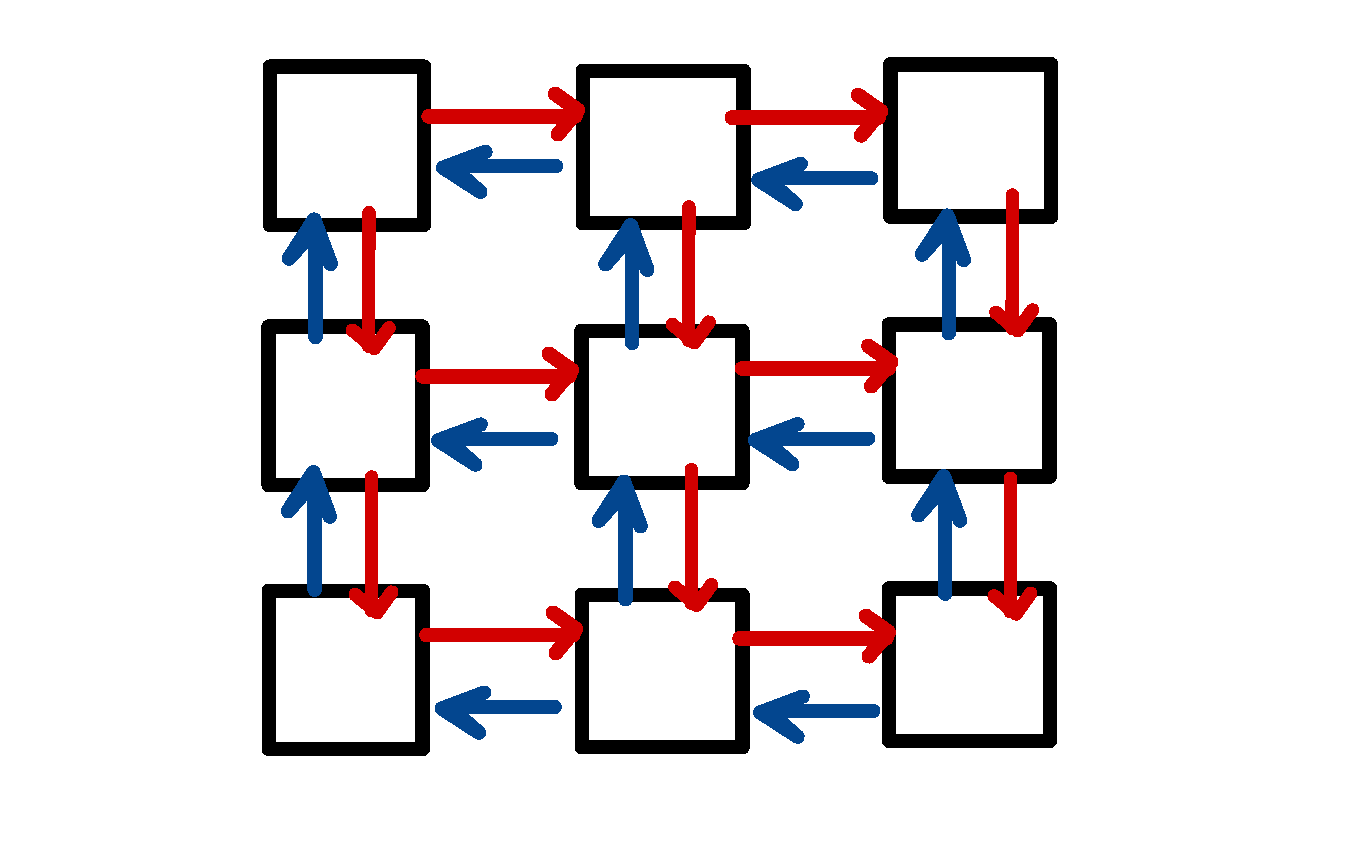
\includegraphics[width=0.9\textwidth]{images/Broadcast.pdf}
\caption{Example of the fully connected routing configuration for a tile (FCT).
Each node represents a digital ASIC which must be aggregated, and the red and blue connections distinguish directions of communication.
The red connection lines indicate pathways away from the base node, whereas the blue lines represent connection paths towards the base-node in the upper-left.
The FCT can be viewed as a directional, weighted graph where the edges are the Tx and Rx connections between ASICs (nodes).
}
\label{fig:fc_tile}
\end{figure}

To elaborate on the adjacency matrix of the FCT we consider an $2\times 3$ tile.
A $2\times 3$ tile has six total nodes, where we consider the upper-left most node to be the base node.
Then, the unweighted adjacency matrix has dimensions $6\times6$ of the form:
\begin{equation}~\label{eq:adjacency_matr}
M =
 \begin{pmatrix}
 0 & 1 & 0 & 1 & 0 & 0 \\
 1 & 0 & 1 & 0 & 1 & 0 \\
 0 & 1 & 0 & 0 & 0 & 1 \\
 1 & 0 & 0 & 0 & 1 & 0 \\
 0 & 1 & 0 & 1 & 0 & 1 \\
 0 & 0 & 1 & 0 & 1 & 0 \\
 \end{pmatrix}
\end{equation}

Where each non-zero value of $M_{ij}$ represents a connection between nodes $i$ and $j$.
As an unweighted, undirected graph this is a symmetric matrix.

In practice each digital channel within a tile is actually controlled by a unique, free-running oscillator.
Therefore, we can define the length of each edge between nodes as the length of time to send of a packet of data between two nodes ($T_{i\rightarrow j}$).
With this we can extend the model the adjacency matrix to a weighted and directed graph if we recognize that the non-zero elements of $M_{ij}$ become $T_{i\rightarrow j}$, or the length of time it takes for the $i^{th}$ local oscillator to transmit a packet to node $j$.

We can generalize this matrix in terms of an arbitrary number of rows ($r$) and columns ($c$).
We define a convention of numbering nodes within the tile in terms of increasing column number followed by increasing row number.
With this convention we obtain the general adjacency matrix with values defined by:
\begin{equation}~\label{eq:adjacency_comp}
  M_{ij} = T_{i\rightarrow j}(\delta_{i,j=i\pm 1} + \delta_{i,j=i\pm r})
\end{equation}

An adjacency list can similarly be constructed from Equation~\ref{eq:adjacency_comp} where the non-zero connections are given by the Kronecker deltas factors.

The length between the nodes represents the time it takes for a packet to transact from one node to the next.
This is determined by both the number of clocks to be sent in the communication protocol ($N_{bits}$) and the period of the transmitting and receiving oscillators, $T_{i}$ and $T_{j}$, respectively.
Unlike the transmitter, the receiver only affects the transaction time with a single clock cycle, as the protocols we test here, (UART and Endeavor), each conclude a packet transaction when the receiver records the last bit transaction from the transmitter.

The full length between two nodes, $i$ and $j$, connected by an edge is represented by:
\begin{equation}~\label{eq:t_packet_full}
T_{i\rightarrow j} = N_{bits}T_{i} + T_{j}(t)
\end{equation}

Where $T_{j}(t)$ represents the time dependent fractional part of one nominal clock period of the receiving node.
The expectation value of $T_{j}(t)$ is half of the nominal window so that mean Equation~\ref{eq:t_packet_full} is:
\begin{equation}~\label{eq:t_packet_avg}
\bar{T}_{i\rightarrow j} \simeq N_{bits}T_{i} + \frac{T_{j}}{2}
\end{equation}

Since the transaction time of a packet is much larger than a single clock cycle ($N_{bits} \simeq \mathcal{O}(10^{2}) \gg \frac{1}{2}$), we can approximate Equation~\ref{eq:t_packet_avg}:
\begin{equation}~\label{eq:t_packet}
\bar{T}_{i\rightarrow j} \approx N_{bits}T_{i}
\end{equation}

This representation is also useful to model certain SPF where a node becomes inactive.
Dead or inactive nodes are ones in which all of their connections are effectively disconnected.
This is equivalent to setting their transaction lengths to zero: $T_{SPF} = 0$.

We comment that although it is possible to construct tiles where more than one node connects to the aggregator, we observe that this configuration simply produces two (or more) effective tiles.
These distinct tiles then are the data paths which are unique to each base-node.
In this graphical representation a packet of data can follow one, and only one path from the origin node to the base-node unless there was duplication of packets.
We emphatically avoid designs which might depend on data duplication for redundancy; situations with multiple base nodes produce multiple unconnected graphs.

\subsubsection{The SPF Cost}\label{sec:spf_cost}
We define the average SPF cost as the amount of nodes that will be lost during a transaction as the number of digital channels at a height below the failed digital channel.
For example, the number of nodes which are lost if a leaf-node fails is one since no other channels are between it and the data node.
Likewise, the number of nodes which are lost in the event of a base-node failure is the total tile, $N$.

We can then calculate a mean cost SPF, $C_{SPF}$, :
\begin{equation}~\label{eq:cspf}
  C_{SPF} = \frac{1}{N}\sum_{node} \frac{n_{i}}{N} = \frac{1}{N^{2}}\sum_{node} n_{i}
\end{equation}

\subsubsection{Minimize Occupancy}\label{sec:min_conn}
One of the goals of a successful digital design is to ensure lossless data transfer.
One point of failure on the digital side is an overabundance of data arriving at a single layer within the tree.
This data loss occurs when data are sent to a node faster than the data leaves the node, and persists for long enough such that the buffers of the node overflow.
This creates a horrible loss of data which can't be recovered.

A routing scheme which minimizes the overall occupancy in the tree depths is shown in Figure~\ref{fig:snake}.
We refer to the style of routing as ``Snake''-routing, because this is also the longest possible routing scheme for a square tile.

\begin{figure}[]
\centering
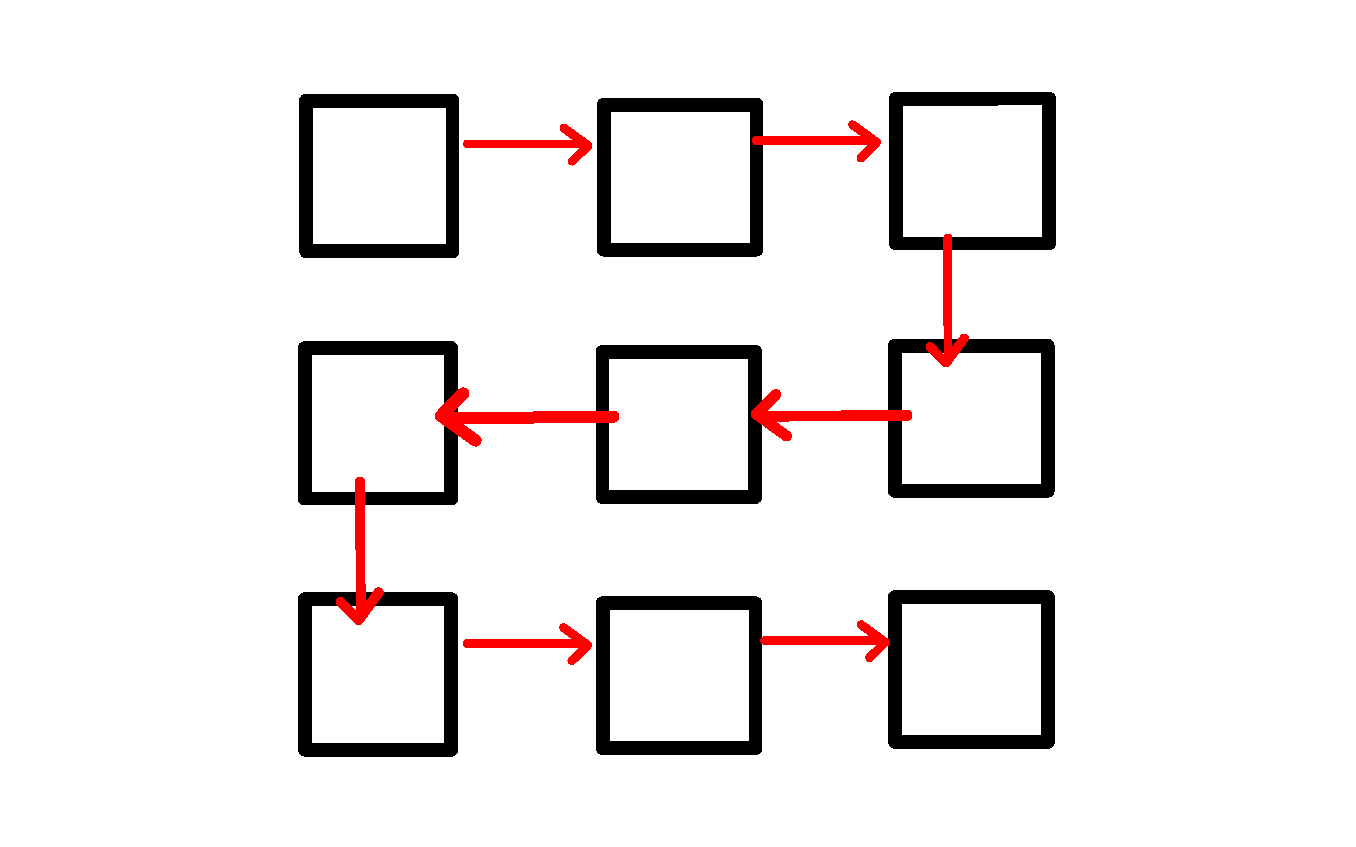
\includegraphics[width=\textwidth]{images/snakeroute.pdf}
\caption{Minimal Occupancy Path of a FCT, or "Snake" routing.
This routing path ensures that the number of input connections equal the number of output paths for the node.}
\label{fig:snake}
\end{figure}

We inspect the SPF risk from this routing scheme with Equation~\ref{eq:cspf}, where we notice that the $n_{i}$ of each node is simply a running sum from the leaf to $N$ at the base node.

\begin{equation}~\label{eq:cspf_snake}
  C_{SPF} = \frac{1}{N^{2}}\frac{N(N+1)}{2} = \frac{1}{n}\frac{N+1}{2} = \frac{1}{2} + \frac{1}{2N}
\end{equation}

Equation~\ref{eq:cspf_snake} tells us that the SPF risk of this routing configuration converges to half as the size of the tile grows.
Intuitively, this makes sense, since it is equally likely to select a node close to the base-node as it is far away, which implies that the sum should converge to half the tile size for large $N$.

Although this routing scheme provides the most lax constraint on the required buffers at each digital channel, it provides the longest average path between the base node.
The longer the transaction delay between the base-node and other nodes increases the reconstruction time uncertainty.
Therefore, a natural alternative routing scheme is one that minimizes the communication scheme.

\subsubsection{Minimize Delay}
\label{sec:min_comm}
For any given node in an edge FCT with location $(R_{i},C_{i}$), the shortest path to the base-node is simply the sum of its coordinates: $R_{i}+C_{i}$.
An example of such a routing configuration for a tile is shown in Figure~\ref{fig:leftroute}.

\begin{figure}[]
\centering
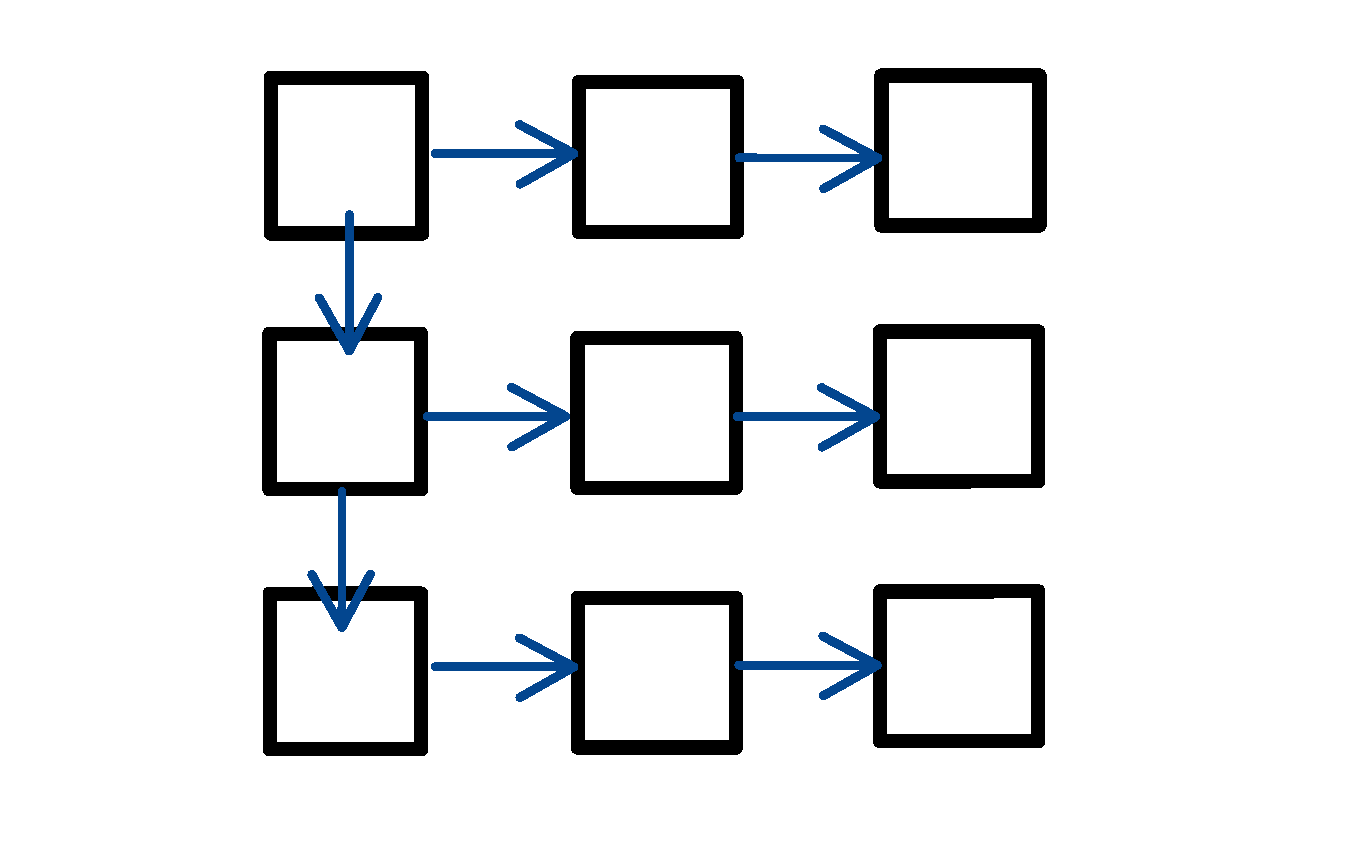
\includegraphics[width=\textwidth]{images/leftroute.pdf}
\caption{Minimal Delay Path of a FCT, or "Left" routing.
This routing path ensures that the minimum number of transactions occur from every node in the FCT to reach the base-node.
For any node along any column this is equivalent to the sum of the row and column of that node.}
\label{fig:leftroute}
\end{figure}

We can calculate $C_{SPF}$ for this routing configuration if we identify that there are a $C$ number of rows which sum from one to $R-1$.
Likewise, the far-left column in Figure~\ref{fig:leftroute} shows that the number of rows, $R$, sum from one to $C$.
We can rewrite the sum over all nodes in Equation~\ref{eq:cspf} as:

\begin{equation}~\label{eq:cspf_left_s}
  \sum_{node}n_{i} = C\sum_{i=0}^{i=R-1}i + R\sum_{i=0}^{i=C}i
\end{equation}

We simplify the running sum of each term in Equation~\ref{eq:cspf_left_s}:
\begin{equation}~\label{eq:cspf_left_e}
  \sum_{node}n_{i} = C\frac{R(R-1)}{2} + R\frac{C(C+1)}{2} = RC(\frac{R+C}{2})
\end{equation}

Using this result we obtain $C_{SPF}$ by identifying $N = RC$:
\begin{equation}~\label{eq:cspf_left_fin}
  C_{SPF} = \frac{1}{N^{2}}\sum_{node}n_{i} = \boxed{\frac{R+C}{2RC}}
\end{equation}

This result informs that relative cost of losing a node tends to zero as the size of the tile grows.
Again, this result can be obtained intuitively, since as the number of columns (or rows) grow in size, the probability of a single failure occurring on the aggregator column is increasingly less likely.

\subsubsection{Broadcasts to avoid SPF}\label{sec:broadcast}
In order to protect against SPF we consider a design which implements the FCT.
A FCT allows searches to probe all possible paths to any node via a ``broadcast'' produced from packets sent by the aggregator to the base-node.
Therefore the broadcast algorithm can be represented by a complete circuit which begins at the base-node and proceeds to a target node with no repeated nodes until the target node is reached.
The backward path is then completed in reverse by following the edges (Tx and Rx connections) between each node until arriving finally again at the base-node.

In practice, broadcasts are encoded as a register request~(Table~\ref{table:node_registers}) created at the aggregator node where Bit 53 (~\ref{fig:datum}) is set to '1'. 
To differentiate between broadcasts an identification number is also included in the packet.
Then, any node when receives a broadcast packet will record the identification number of the most recent broadcast, and send this packet to its connected neighbors in the direction it did not receive the broadcast.
The node uses the identification number to discard repeated broadcast packets.

In the event that a particular node becomes inactive it will ``block'' data coming from the nodes along its path.
In this case, there must be some sort of ``broadcast'' originating from the base-node that would allow information transverse regardless of the effective routing path.

%% colored matrix
\def\r{\color{red}1}
\def\b{\color{blue}1}
\begin{figure}[h]
  \begin{tabular}{p{5cm}c}
    {${\renewcommand{\arraystretch}{2.0}}
        \begin{pmatrix}
          0 & \r & 0 & \r & 0 & 0 \\
          \b & 0 & \r & 0 & \r & 0 \\
          0 & \b & 0 & 0 & 0 & \r \\
          \b & 0 & 0 & 0 & \r & 0 \\
          0 & \b & 0 & \b & 0 & \r \\
          0 & 0 & \b & 0 & \b & 0 \\
        \end{pmatrix}$}
    &
    $\vcenter{\hbox{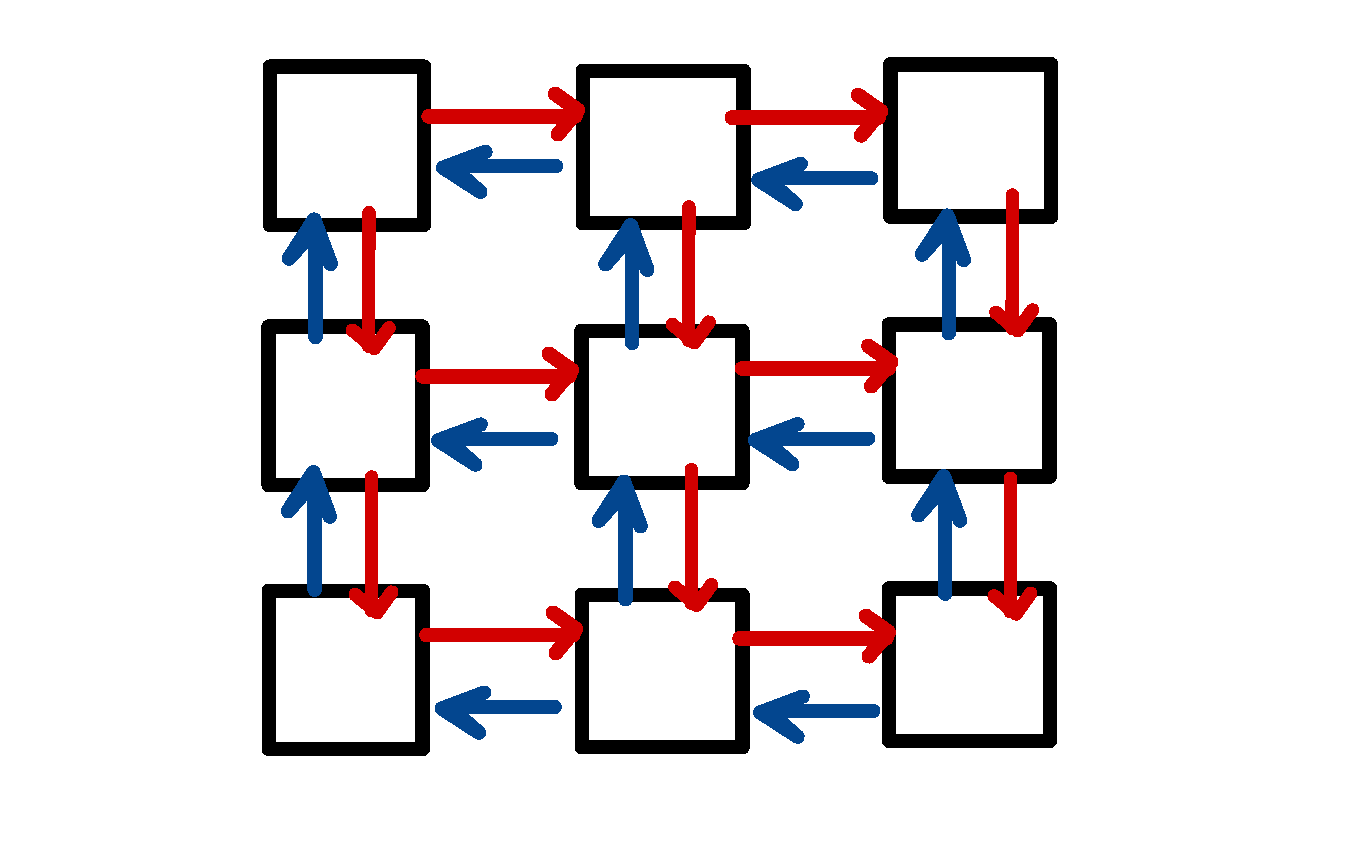
\includegraphics[scale=0.45]{images/Broadcast.pdf}}}$
  \end{tabular}
\caption{Minimal Routing Path of a FCT.
This routing path ensures that the number of input connections equal the number of output paths for the node.
The matrix image highlights the appropriate indices which correspond to the 2$\times$3 subset of the tile (right).
The matrix represents transactions that proceed towards (red) and away from (blue) the base node.
}
\label{fig:FCT_colored}
\end{figure}

\subsection{Comments on the Edge Base-node and Other Routings}\label{sec:base_node}
We discuss here the case of a FCT with an edge base node.
An edge base node (EBN) is a node which connects to the aggregator and to three other digital channels within a tile.
An example of an EBN is shown in Figure~\ref{fig:ebn}.
Like before, this base-node must provide a unique path during data transmission to all digital channels within the tile.
In this configuration the adjacency matrix is still the same as given in Equation~\ref{eq:adjacency_comp}.

\begin{figure}[]
\centering
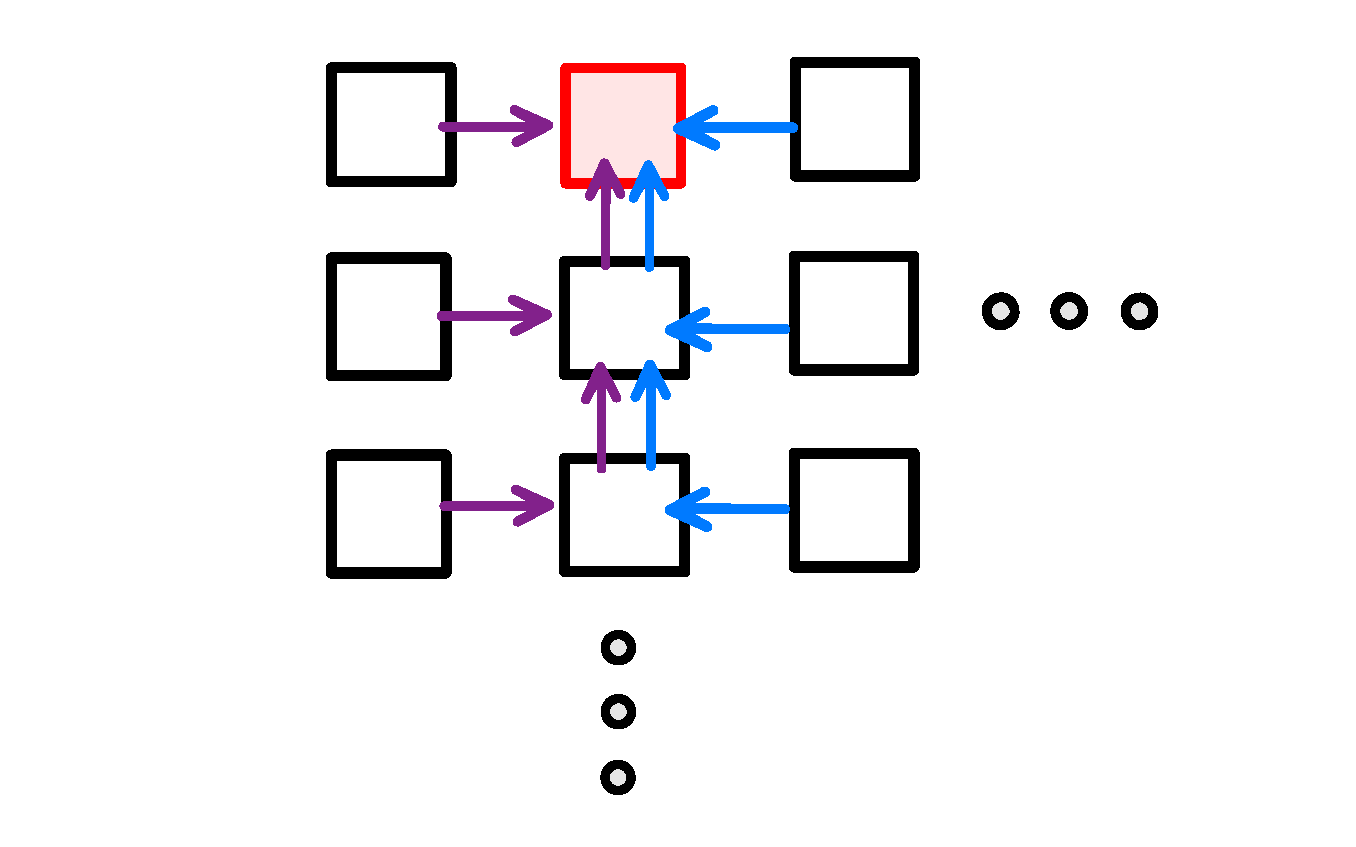
\includegraphics[width=0.8\textwidth]{images/EBN_superposition.pdf}
\caption{Example of an Edge base-node configuration.
The base-node is colored and highlighted in red.
Image shows how the EBN can be thought of as a super-position of two corner base-nodes, represented by the purple (left "tile") and blue (right "tile") connections.
Instead of a 3$\times$3 tile, there are two 2$\times$3 "tiles".
}
\label{fig:ebn}
\end{figure}
